\documentclass{entcs} 
\usepackage{entcsmacro}
\usepackage{graphicx}
\sloppy
% The following is enclosed to allow easy detection of differences in
% ascii coding.
% Upper-case    A B C D E F G H I J K L M N O P Q R S T U V W X Y Z
% Lower-case    a b c d e f g h i j k l m n o p q r s t u v w x y z
% Digits        0 1 2 3 4 5 6 7 8 9
% Exclamation   !           Double quote "          Hash (number) #
% Dollar        $           Percent      %          Ampersand     &
% Acute accent  '           Left paren   (          Right paren   )
% Asterisk      *           Plus         +          Comma         ,
% Minus         -           Point        .          Solidus       /
% Colon         :           Semicolon    ;          Less than     <
% Equals        =3D           Greater than >          Question mark ?
% At            @           Left bracket [          Backslash     \
% Right bracket ]           Circumflex   ^          Underscore    _
% Grave accent  `           Left brace   {          Vertical bar  |
% Right brace   }           Tilde        ~

% A couple of exemplary definitions:

\newcommand{\Nat}{{\mathbb N}}
\newcommand{\Real}{{\mathbb R}}

\def\lastname{Martins Moreira}

\begin{document}
\begin{frontmatter}
%  \title{Modeling the Java Card API (or Interface?) in B} \author{A. Martins Moreira\thanksref{ALL}\thanksref{anamaria}}
%  \address{DIMAp-UFRN, Natal, RN, Brazil} \author{S. de Oliveira Santos \thanksref{simone}}
%  \address{DIMAp-UFRN, Natal, RN, Brazil} \author{B. Emerson Gurgel Gomes \thanksref{bruno}}
%    \address{IFRN, Currais Novos, RN, Brazil} \author{D. Boris Paul D\'{e}harbe \thanksref{david}}
%      \address{DIMAp-UFRN, Natal, RN, Brazil} \thanks[ALL]{INES-CAPES-projeto GD?... o que mais?} \thanks[anamaria]{Email:
%    \href{mailto:anamaria@dimap.ufrn.br} {\texttt{\normalshape
%        anamaria@dimap.ufrn.br}}} 
%      \thanks[simone]{Email:
%    \href{mailto:simone82@ppgsc.ufrn.br} {\texttt{\normalshape
%        simone82@ppgsc.ufrn.br}}}
%      \thanks[bruno]{Email:
%    \href{mailto:bruno.gurgel@ifrn.edu.br} {\texttt{\normalshape
%        bruno.gurgel@ifrn.edu.br}}}
%       \thanks[david]{Email:
%    \href{mailto:david@dimap.ufrn.br} {\texttt{\normalshape
%        david@dimap.ufrn.br}}}

  \title{Modeling the Java Card API (or Interface?) in B} \author[ufrn]{A. Martins Moreira\thanksref{ALL}\thanksref{anamaria}}
  \author[ufrn]{S. de Oliveira Santos \thanksref{simone}}
  \author[ifrn]{B. Gurgel Gomes \thanksref{bruno}}
  \author[ufrn]{D.  D\'{e}harbe \thanksref{david}}
  \address[ufrn]{DIMAp-UFRN, Natal, RN, Brazil} \thanks[ALL]{INES-CAPES-projeto GD?... o que mais? REUNI?}  \address[ifrn]{IFRN, Currais Novos, RN, Brazil} 
 \thanks[anamaria]{Email:
    \href{mailto:anamaria@dimap.ufrn.br} {\texttt{\normalshape
        anamaria@dimap.ufrn.br}}} 
      \thanks[simone]{Email:
    \href{mailto:simone82@ppgsc.ufrn.br} {\texttt{\normalshape
        simone82@ppgsc.ufrn.br}}}
      \thanks[bruno]{Email:
    \href{mailto:bruno.gurgel@ifrn.edu.br} {\texttt{\normalshape
        bruno.gurgel@ifrn.edu.br}}}
       \thanks[david]{Email:
    \href{mailto:david@dimap.ufrn.br} {\texttt{\normalshape
        david@dimap.ufrn.br}}}


\begin{abstract} 
  The B method development process starts from an abstract model of a
  set of services that are to be developed, and includes formally
  verified refinements, which introduce implementation details. At a
  final refinement step these implementation details depend on the
  language for which code is to be generated. To rigorously develop
  Java Card Applications with the B method, then, it is necessary to
  model in B the constructs of Java Card, so that the gap between the
  B formally verified implementation model and the Java Card generated
  code is as small as it can be. In the context of the BSmart project,
  we have developed the specification of the Java Card Application
  Programming Interface (Java Card API), to be used in the development
  of Java Card applications with B.
\end{abstract}
\begin{keyword}
  Java Card, smart cards, B method, formal methods
\end{keyword}
\end{frontmatter}
\section{Introduction}\label{intro}

In the context of the BSmart project, we are interested in the use of
B to develop Java Card~\cite{chen:2000} applications.  Java Card is a
restricted and optimized version of Java which allows memory and
processor constrained devices, such as smart cards, to store and run
small applications.  Java Card applications have characteristics
(small size and need for security) which make them good candidates for
formal development with the B method. They also present some
regularity of structure that induced our group into the definition of
a method and a tool which specialize B for development of such
applications, providing greater support for the developer than pure B
tools \cite{atelierB,proB}. They are the BSmart method and tool,
presented in \cite{BSmart08,Gomes10}.

Previous works have also dealt with B for Smart Cards, 
\cite{Bert:2003,JBtools,tatibouet:lncs,requetBtoC}, but none has, at our knowledge, specified Java Card
in B so that the formal development includes Java Card aspects. In the
first versions of BSmart \cite{Gomes10}, these aspects were included by the code
generator, and in JBTools \cite{JBtools}, the generated code needed to be edited by
the developer to include these aspects.

These works lacked then the ability to formally verify the Java Card dependent aspects of the application. To be able to change this, a B
specification of these aspects is needed, and this contribution is what we present in this paper: the B specification of the Java Card
API, with its primitive types and all classes of the 14 packages which define the API. This specification can be used with the BSmart tool,
independently, in any B tool, or even as a complement to the official Java Card documentation \cite{oracle}.

In the following...

\section{Smart Cards and Java Card}\label{sec:javacard}


AMM: TRECHOS EXTRAIDOS E JA UM POUCO ALTERADOS DO ABZ 2010. DEPENDENDO
DO QUE VAMOS MOSTRAR NA ESPECIFICA�AO PODEMOS DEIXAR MAIS OU MENOS
DETALHES AQUI. NO FINAL, PRECISAMOS VERIFICAR QUE NAO COPIAMOS DEMAIS
O QUE ESTAVA LA.

A smart card application is distributed between on-card and off-card
components.  The server application on the card side (called applet)
provides the application services. The off-card client (called host
application) resides in a computer or electronic terminal.

The information exchange between the host and card applications is
made through a a half-duplexed low level protocol, named
\emph{Application Protocol Data Unit} (APDU).  The ISO 7816-4 standard
specifies two kinds of APDU's, which are the command and the response
APDU (Figure~\ref{fig:APDUs}). Both specify data packets. A command APDU
is sent by the host, requiring some applet service and a response APDU is
sent by the applet, responding to the host request with the result of the
service processing.

\begin{figure}[!ht]
\centering
%\includegraphics[scale=0.3]{figs/comandoAPDU.jpg}
%\includegraphics[scale=0.3]{figs/respostaAPDU.jpg}
\caption{Command and response APDUs. Source:~\cite{ortiz1intro:2003}}
\label{fig:APDUs}
\end{figure}

The main component of the Java Card platform (Figure~\ref{fig:jcre})
is its runtime environment (JCRE), composed of a Java Card Virtual
Machine (JCVM), an API, and, usually, system and
industry-specific classes~\cite{chen:2000}. The JCRE acts as a small
operating system, being responsible for the control of the application
lifetime, security and resource management.

\begin{figure}[h]
\centering
%\includegraphics[width=0.35\textwidth]{figs/jcplatform.png}
\caption{Java Card platform components. Adapted from:~\cite{ortiz1intro:2003}}
\label{fig:jcre}
\end{figure}


\paragraph{Java Card applets}\label{sec:applets}

A Java Card applet is a class that inherits the
\emph{javacard.framewok.Applet} class of the Java Card API and is
implemented upon the Java Card subset of Java.  During the applet
conversion for card installation, a verification phase is performed to
check conformance of the classes with Java Card restrictions.

The current usual Java Card specification (2.2.x) allows two kinds of
applets.  The older, and most commonly used, kind of applet manipulates
directly the APDU protocol packages while the newer one abstracts from
the lower level protocol using Remote Method Invocation (RMI). In this
paper we will call the lower level applet \emph{APDU applet} and the
higher level one, \emph{RMI applet}. RMI introduces a layer of
abstraction above the APDU protocol, and, due to this fact, it is usually
less efficient than APDU applets.


\section{B specification of the Java Card API}

Among the different components of the Java Card platform, the Java Card API is the one without which no refinement into Java Card code could be done.
Suppose, for instance, that we had the B abstract machine of Fig. \ref{fig:Bmachine}, which models a bus card with a variable that controls balance and a operation to add credits to the balance. Of course, this is a very simple example, but it is enough to show the importance of having the model of the Java Card API modeled in B.  As all data in it is implementable in C, for instance, and it is a deterministic specification, B tools can directly generate code for it in C, and the resulting code would be very similar to the original B machine.

\begin{figure}[h]
\centering
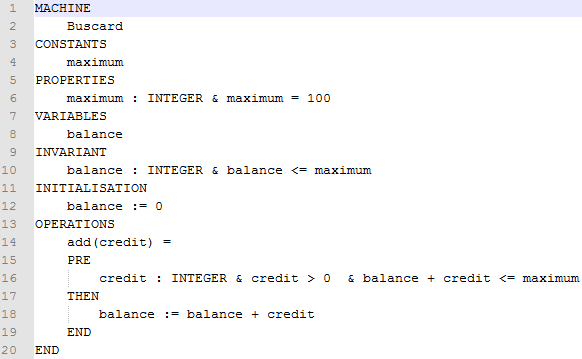
\includegraphics[width=0.8\textwidth]{figs/machineB.png}
\caption{Example B machine.}
\label{fig:Bmachine}
\end{figure}

However,  Java Card code corresponding to it would look like the one presented in Fig. \ref{fig:jcapplet}. In a rigorous development process, we don't want the code generator to carry out all these non-verified transformations in the code. So, we need to be able to refine the original B machine into something such as the B refinement of fig. \ref{B ref usando a API}. Then, code generation would be straightforward, as it should be. This is then the reason why it needed to be the first Java Card component to be modeled in B. (AMM: maybe also cite related work ? WHich are the formalization works that did not focus on the API?)


\begin{figure}[h]
\centering
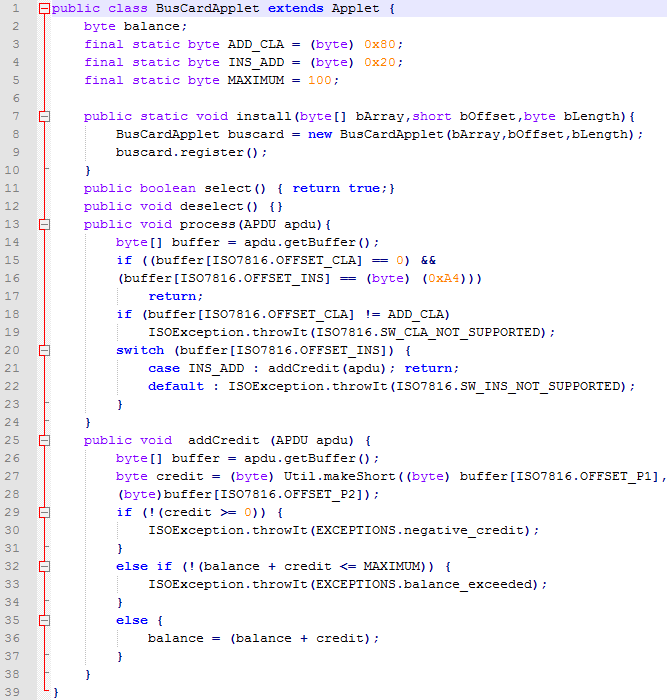
\includegraphics[width=0.8\textwidth]{figs/appletJC.png}
\caption{Example Java Card applet.}
\label{fig:jcapplet}
\end{figure}


COMENT SIMONE -> coloquei duas figuras, veja o que acha do exemplo, � o mesmo que foi usado na disserta��o, ele � simples e pequeno. Coloquei a m�quina abstrata e o modelo do applet Java Card (veja o que acha do tamanho das figuras), estou vendo com o Bruno como a implementa��o desta m�quina fica com a API, porque o modelo dela que fizemos foi sem o uso da API, ela possui apenas o uso dos tipos primitivos e as opera��es de soma e compara��o deles. O exemplo que n�s usamos na valida��o do trabalho que tinha o uso da API foi um refinamento da m�quina applet.

PARA SIMONE -> Por favor, coloque os exemplos sob a forma de listing. Fica mais f�cil de editar, controlar o tamanho e conte�do e fica mais leg�vel.
Quanto ao c�digo javacard, basta o da opera��o addcredit. Ali�s, o nome n�o est� batendo. N�o verifiquei o resto. Por favor verifique.


The Java Card API, in its version 2.2.2, is defined in 14 packages, containing 93 classes and interfaces, as shown in Table \ref{tab:packages}. Their interfaces have all been modeled in B, and the resulting models are available at the KitSmart project page\footnote{https://code.google.com/p/kitsmart/}. Differently from  JML and OCL, though, B is not object oriented, and some modeling solutions had to be found to cope with this lack of resources.  We present in the following the main characteristics and restrictions of our models:

\begin{table}[h]
\begin{center}
\caption{Packages of the Java Card API (2.2.2) and the number of classes in each package.}
\begin{tabular}{|l|c||l|c|}
 \hline
 
\textbf{\small{Package}} & \textbf{\small{classes}} & \textbf{\small{Package}} & \textbf{\small{classes}}\\ \hline \hline
\small{java.io} & \small{1} & \small{javacardx.biometry} & \small{5} \\ \hline
\small{java.lang} & \small{12} & \small{javacardx.crypto }& \small{2} \\ \hline
\small{java.rmi} & \small{2} & \small{javacardx.external} & \small{3} \\ \hline
\small{javacard.framework} & \small{19} & \small{javacardx.framework.math} & \small{3} \\ \hline
\small{javacard.framework.service} & \small{8} & \small{javacardx.framework.tlv} & \small{7} \\ \hline
\small{javacard.security} & \small{27} & \small{javacardx.framework.util} & \small{2} \\ \hline
\small{javacardx.apdu} & \small{1} & \small{javacardx.framework.util.intx} & \small{1} \\

 \hline
\end{tabular}
\label{tab:packages}
\end{center}
\end{table}

\begin{itemize}

\item Only the abstract models corresponding to each class or interface have been developed. Two reasons led to this choice: (1) code is not to be generated from the specification of the API, as we are only creating an abstract layer to existing implementations; and (2)  in B, only the abstract machines are seen by modules that build upon others, through the SEES, USES, IMPORTS, INCLUDES and EXTENDS clauses.

\item Conditions on method inputs which lead to exception raising in the Java Card platform specification are coded into pre-conditions in B.
(em que casos isso n�o � feito - NULL? outros?)

\item Method outputs are modeled in B as taking any value of the correct type (e em que casos temos um pouco mais).





\end{itemize}



\section{Using the model in BSmart}


\section{Conclusions}



\bibliographystyle{plain}
\bibliography{bib}

\end{document}
